\documentclass{article}

\usepackage{graphicx} %[pdftex] OR [dvips]
\usepackage{fullpage}
\usepackage{float}
\usepackage{titling}
\setlength{\droptitle}{-6em}

\newcommand{\ghcfile}[1]{\textsl{#1}}

\title{Implementing Backpack}

\begin{document}

\maketitle

The purpose of this document is to describe an implementation path
for Backpack~\cite{Kilpatrick:2014:BRH:2535838.2535884} in GHC\@.

We start off by outlining the current architecture of GHC, ghc-pkg and Cabal,
which constitute the existing packaging system.  We then state what our subgoals
are, since there are many similar sounding but different problems to solve.  Next,
we describe the ``probably correct'' implementation plan, and finish off with
some open design questions.  This is intended to be an evolving design document,
so please contribute!

\section{Current packaging architecture}

The overall architecture is described in Figure~\ref{fig:arch} (ignore
the red and green bits for now).

\begin{figure}[H]
    \center{\scalebox{0.8}{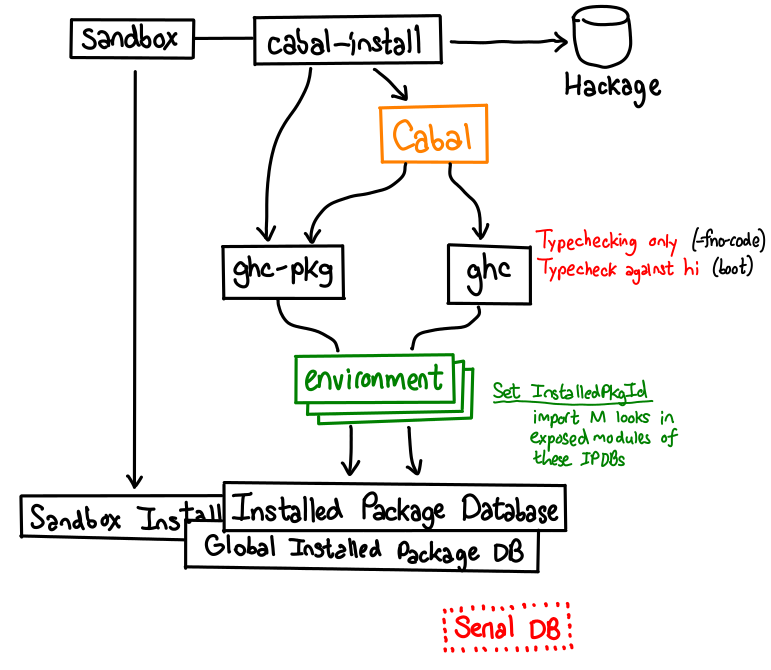
\includegraphics{arch.png}}}
\label{fig:arch}\caption{Architecture of GHC, ghc-pkg and Cabal. Green bits indicate additions from upcoming IHG work, red bits indicate additions from Backpack.  Orange indicates a Haskell library.}
\end{figure}

Here, arrows indicate dependencies from one component to another.
(insert architectural description here)

A particularly important component of this picture is the package
database, sketched in Figure~\ref{fig:pkgdb}.

\begin{figure}[H]
    \center{\scalebox{0.8}{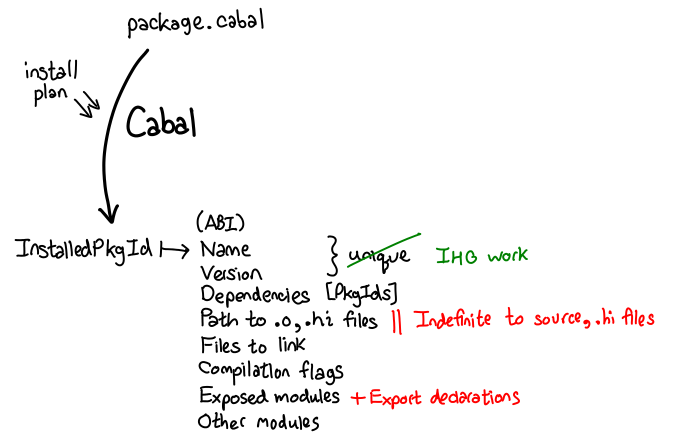
\includegraphics{pkgdb.png}}}
\label{fig:pkgdb}\caption{Anatomy of a package database and a package identifier.}
\end{figure}

An installed package is calculated from a Cabal file through the process
of dependency resolution and compilation.  We can think of it a
database, whose primary key is the InstalledPackageId, which presently
is the package name, the package version, and the ABI hash (nota bene,
the diagram disagrees with this text: it shows the version of installed
package IDs which we'd like to move towards.)  These IDs uniquely
identify an instance of an installed package.  A mere PackageId omits
the ABI hash.

The database entry itself contains the information from the installed package ID,
as well as information such as what dependencies it was linked against, where
its compiled code and interface files live, its compilation flags, what modules
it exposes, etc.  Much of this information is only relevant to Cabal; GHC
uses a subset of the information in the package database.

\section{Goals}

There are actually a number of different goals we have for modifying the
packaging system.

\begin{itemize}
    \item Support multiple instances of containers-2.9 \emph{in the
        package database}.  These instances may be compiled against
        different dependencies, have the same dependencies but different
        source files (as when a package is being developed), or be
        compiled with different options.  It is less important to allow
        these instances to be linkable together.

    \item Some easy-to-implement subset of the functionality provided by
        packages with holes (Backpack proper).
\end{itemize}

A lower priority goal is to actually allow multiple instances of
containers-2.9 to be linked together in the same executable
program.\footnote{In particular, this requires changes to how linker symbols
are assigned. However, this feature is important to implement a number
of Backpack features.}

A \emph{non-goal} is to allow users to upgrade upstream libraries
without recompiling downstream. This is an ABI concern and we're not
going to worry about it.

\section{Aside: Recent IHG work}

The IHG project has allocated some funds to relax the package instance
constraint in the package database, so that multiple instances can be
stored, but now the user of GHC must explicitly list package-IDs to be
linked against.  In the far future, it would be expected that tools like
Cabal automatically handle instance selection among a large number of
instances, but this is subtle and so this work is only to do some
foundational work, allowing a package database to optionally relax the
unique package-version requirement, and utilize environment files to
select which packages should be used.  See Duncan's email for more
details on the proposal.

For the purpose of Backpack, the only relevant part of this proposal
is the relaxation of package databases to allow multiple 

\section{Adding Backpack to GHC}

Backpack additions are described in red in the architectural diagrams.
The current structure of this section is to describe the additions bottom up.

\subsection{Use InstalledPackageId instead PackageId in typechecking}

In Backpack, there needs to be some mechanism for assigning
\emph{physical module identities} to modules, which are essential for
typechecking Backpack packages, since they let us tell if two types are
equal or not. In the paper, the physical identity was represented as the
package that constructed it as well as some representation of the module
source.  We can simplify this slightly: in current Cabal packages, we
require that modules always be given a package-unique logical name;
thus, physical identities can be simply represented as a PackageId plus
module name. (See \ghcfile{compiler/basicTypes/Module.lhs:Module})

However, this is not enough if we allow multiple instances of a package
in the package database: now we may incorrectly conclude that types
defined by different instances of the same version of a package are
equal: this would be especially fatal if the two packages were linked
against different underlying libraries.  Thus, a physical module name
should be represented as an InstalledPackageId (which uniquely
identifies an installed package) as well as the original logical name.

\paragraph{Note about linker symbols} Module is currently used for
typechecking, and then once again

Currently, InstalledPackageId is constructed of a package, version and ABI
hash.  The use of an ABI hash is a bit of hack, mostly to make sure these
installed package IDs are unique.  In Figure~\ref{fig:pkgdb}, an alternate
logical representation of InstalledPackageId is suggested using 

----

Simon gave some nice explanations of original names in GHC

Sometimes, a name can be exposed in an hi file even if its module
wasn't exposed. Example in package R:

    module X where
    import Internal (f)
    g = f

    module Internal where
    import Internal.Total (f)

Then in X.hi:

    g = <R.id, Internal.Total, f> (this is the original name)

(The reason we refer to the package as R.id is because it's the
full package ID, and not just R).

How might internal names work with Backpack?

    package P where
        M = ...
        N = ...
    package Q (M, R, T)
        include P (N -> R)
        T = ...

    Q; exposed modules
        M -> <P.id, M>
        R -> <P.id, N>
        T -> <Q.id, T>

When we compile Q, and the interface file gets generated, we have
to generate identifiers for each of the exposed modules.  These should
be calculated to directly refer to the "original name" of each them;
so for example M and R point directly to package P, but they also
include the original name they had in the original definition.

----

Differing intuitions: GHC internals versus Backpack abstraction

----

Refactoring necessary:

    - PackageId in GHC needs to be InstalledPackageId.  I get these IDs
      from -package-name when I build a package, and these are baked
      into the hi files and linker names.  To the type checker, this
      IS exactly what a package is.  But see open question about linker
      names...

        There appears to already be a conversion, probably a newtype,
        from package name to linker names, according to Duncan.

      THE PLAN: To remain BC, we have a flag named -package-name which
      is used for both.  So now I maintain two different values,
      -package-name sets both, and then I have another flag for setting
      one separately.

      Watch out: GHC plays tricks with wired-in names. Suggested is a
      table from wired names to package IDs (constructed with the
      package environment)

ghc-pkg

    - Remove the "removal step" when registering a package (with a flag)

    - Check main/Packages.lhs:mkPackagesState to look out for shadowing
      within a database, it might already do the right thing (key idea
      is that we already do something sensible merging package databases
      together, reuse that)

    - Experiment using -hide-all-packages -package-id ... flags explicitly

\section{Open questions}

Here are open problems about the implementation which still require
hashing out.

    - Aliasing of signatures means that it is no longer the case that
      original name means type equality.  We were not able to convince
      Simon of any satisfactory resolution.  Strawman proposal is to
      extending original names to also be variables probably won't work
      because it is so deeply wired, but it's difficult to construct hi
      files so that everything works out (quadratic).

    - Relationship between linker names and InstalledPackageId? The reason
      the obvious thing to do is use all of InstalledPackageId for linker
      name, but this breaks recompilation.  So some of these things
      should go in the linker name, and not others (yes package, yes
      version, yes some compile flags (definitely ways), eventually
      dependency package IDs, what about cabal build flags).  This is
      approximately an ABI hash, but it's computable before compilation.
      This worries Simon because now there are two names, but maybe
      the DB can solve that problem--unfortunately, GHC doesn't ever
      register during compilation; only later.

        Simon also thought we should use shorter names for linker
        names and InstallPkgIds.  This appears to be orthogonal.

    - In this example:

        package A where
            A = [ ... ]
        package A2 where
            A2 = [ ... ]
        package B (B)
            ...

      Do the seperate instantiations of B exist as seperate artifacts
      in the database, or do they get constructed on the fly by
      definite packages which include them?  The former is conceptually
      nicer (identity of types work, closer to Backpack semantics), but
      the latter is easier for linker names. (Simon's first inclination
      is to construct it on the fly.)

      There was another example, showing that we need to solve this
      problem even for indefinite combinations of indefinite modules.
      You can get to it by modifying the earlier example so that C and
      D still have holes, which E does not fill.

    - We have to store the preprocessed sources for indefinite packages.
      This is hard when we're constructing packages on the fly.

    - What is the impact on dependency solving in Cabal?  Old questions
      of what to prefer when multiple package-versions are available
      (Cabal originally only needed to solve this between different
      versions of the same package, preferring the oldest version), but
      with signatures, there are more choices.  Should there be a
      complex solver that does all signature solving, or a preprocessing
      step that puts things back into the original Cabal version.
      Authors may want to suggest policy for what packages should actually
      link against signatures (so a crypto library doesn't accidentally
      link against a null cipher package).

\section{Immediate tasks}

At this point in time, it seems we can identify the following set
of non-controversial tasks which can be started immediately.

\begin{itemize}
    \item Relax the package database constraint to allow multiple
        instances of package-version.
    \item Propagate the use of \verb|InstalledPackageId| instead of
        package IDs for typechecking (but not for linking, yet).
    \item Implement export declarations in package format, so
        packages can reexport modules from other packages.
\end{itemize}

The aliasing problem is probably the most important open problem
blocking the rest of the system.

\bibliographystyle{plain}
\bibliography{backpack-impl}

\end{document}
